\title{Midterm 2 for Algebra-Based Physics-1: Mechanics (PHYS135A-01)}
\author{Dr. Jordan Hanson - Whittier College Dept. of Physics and Astronomy}
\date{October 24th, 2018}
\documentclass[10pt]{article}
\usepackage[a4paper, total={18cm, 27cm}]{geometry}
\usepackage{outlines}
\usepackage[sfdefault]{FiraSans}
\usepackage{graphicx}

\begin{document}
\maketitle

\section{Equations}
\begin{itemize}
\item Newton's First Law: $\vec{F}_{Net} = 0$ if $\vec{v}$ is constant.  Newton's Second Law: $\vec{F}_{Net} = m \vec{a}$. Newton's Third Law: $\vec{F}_{AB} = -\vec{F}_{BA}$.
\item Normal force: $\vec{N} = +mg\hat{y}$, if weight is $w = -mg\hat{y}$ (flat surface).
\item Force of Friction: $\vec{F} = -\mu \vec{N}$ (minus sign: opposes motion).
\item Static versus kinetic friction: $\mu_s \geq \mu_k$.
\end{itemize}

\section{Newton's Laws}
\begin{enumerate}
\small
\item A tree frog leaps sideways from one leaf to another that is several meters below.  As the frog is floating through the air, its webbed feet provide a drag force in the upward direction.  If the frog floats through the air at \textit{constant velocity}, which of the following is true?
\begin{itemize}
\item A: There is a net force on the frog, downwards.
\item B: There is a net force on the frog, upwards.
\item C: There is no net force on the frog, because it is moving at constant velocity.
\item D: There is a net force on the frog, in a horizontal direction.
\end{itemize}
\item A surfer on a surfboard slides along the surface of the ocean, slowing down.  The water provides the normal force that balances her weight.  If we call the direction in which she is moving ``positive,'' in which direction is the net force?
\begin{itemize}
\item A: In the same direction she is moving.
\item B: In the opposite direction she is moving.
\item C: In the upward direction.
\item D: In the downward direction.
\end{itemize}
\item A tractor pulls a palette which slides along a gravel road, causing friction on the palette.  The palette is connected to the tractor by a taught rope.  If the tractor and palette are accelerating, but the rope stays taught, which of the following is true?
\begin{itemize}
\item A: The force of friction on the palette is greater than the tension in the rope.
\item B: The force of friction on the palette is equal to the tension in the rope.
\item C: The force of friction on the palette is greater than the tension in the rope.
\item D: The force of friction on the palette is equal to zero.
\end{itemize}
\item A tractor pulls a palette which slides along a gravel road, causing friction on the palette.  The palette is connected to the tractor by a taught rope.  If the tractor and palette are accelerating, but the rope stays taught, which of the following is true?
\begin{itemize}
\item A: The force of friction on the palette is greater than the tension in the rope.
\item B: The force of friction on the palette is equal to the tension in the rope.
\item C: The force of friction on the palette is greater than the tension in the rope.
\item D: The force of friction on the palette is equal to zero.
\end{itemize}
\item A soccer player strikes a stationary ball with her foot.  Her foot has more mass than the ball.  Which of the following is true?
\begin{itemize}
\item A: The magnitude of the force of her foot on the ball \textbf{is more} than the magnitude of the force of the ball on her foot.
\item B: The magnitude of the force of her foot on the ball \textbf{is less} than the magnitude of the force of the ball on her foot.
\item C: The magnitude of the force of her foot on the ball \textbf{is equal} to the magnitude of the force of the ball on her foot.
\item D: The magnitude of the force of her foot on the ball and the magnitude of the force of the ball on her foot are \textbf{zero}.
\end{itemize}
\clearpage
\item Consider Fig. \ref{fig:car_pull}.  Show that if the applied force F$_{\perp}$ and the tension T balance to 0 N, that $T = F_{\perp}/(2\sin\theta)$. \vspace{2.5cm}
\begin{figure}
\centering
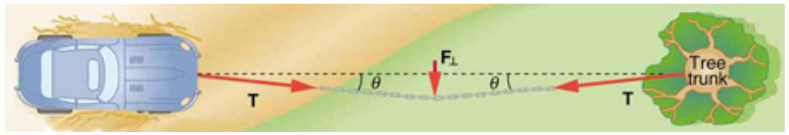
\includegraphics[width=0.6\textwidth]{figures/carpull.png}
\caption{\label{fig:car_pull} Diagram for exercises 3 and 4, \textbf{Newton's Laws.}}
\end{figure}
\item If a person applies F$_{\perp} = 1000$ N, and the angle is $\theta=7^{\circ}$, what is the tension T in the line?  (Use $T = F_{\perp}/(2\sin\theta)$). \vspace{2.5cm}
\item A $5.00\times 10^5$ kg rocket is accelerating upwards with thrust $1.250\times 10^7$ N, but there is also a downward force of $4.5\times 10^6$ N due to air resistance (the rocket also has a weight). (a) Draw a free-body diagram including weight, thrust, and air-resistance.  (b) Calculate the acceleration using Newton's second law. \\ \vspace{2.5cm}
\item Consider Fig. \ref{fig:tug}, in which two tugboats push a barge ($F_x = 2.7\times 10^5$ N, and $F_y = 3.6\times 10^5$ N).  (a) What is the magnitude of the net force on the barge? (b) If the barge has a mass of $5\times 10^6$ kg, what is the acceleration of the barge? \vspace{2.5cm}
\begin{figure}[h]
\centering
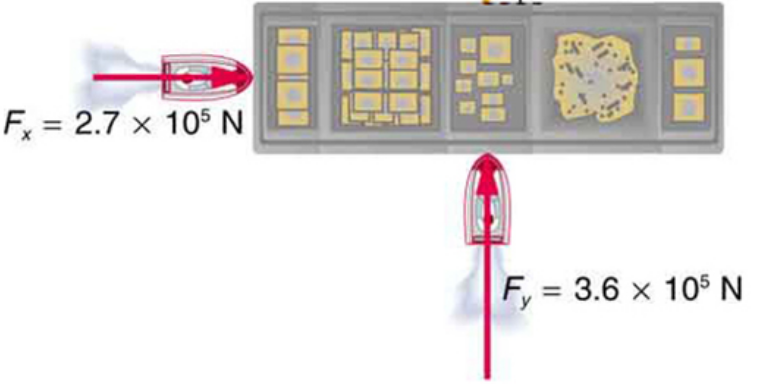
\includegraphics[width=0.4\textwidth]{figures/tug.png}
\caption{\label{fig:tug} Diagram for exercise 6, \textbf{Newton's Laws.}}
\end{figure}
\end{enumerate}
\section{Friction and Drag}
\small
\begin{enumerate}
\item A dog who ``just can't right now'' is being pulled along a ceramic kitchen floor by its human.  The human exerts a force of 20 N horizontally, and the dog has a mass of 20 kg.  If the lazy puppy is moving at a constant velocity, what is the coefficient of kinetic friction $\mu_k$ between the dog and the floor? \\ \vspace{1.5cm}
\item Consult Fig. \ref{fig:coeff}. (a) What is the magnitude of the force of friction on a 1000 kg vehicle on rubber tires, skidding across dry concrete? (b) What would be the new magnitude of the force of friction if the concrete was wet? (c) What is the magnitude of the force of friction on a 60 kg snowboarder sliding across wet snow on a waxed snowboard? \\ \vspace{1.5cm}
\begin{figure}
\centering
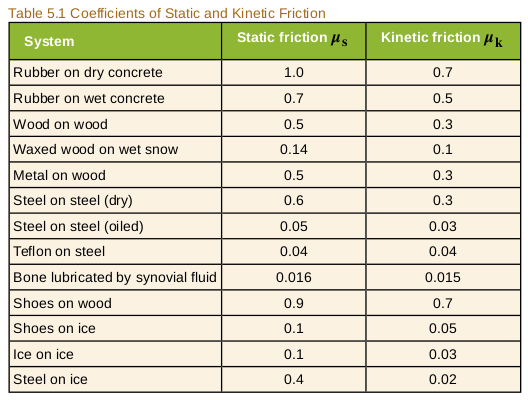
\includegraphics[width=0.55\textwidth]{figures/coefficients.png}
\caption{\label{fig:coeff} (Left) Frictional coefficients for exercise 2, \textbf{Friction and Drag}.}
\end{figure}
\item Consult Fig. \ref{fig:blocks}.  If $m_1 = 1000$ grams, and $m_2 = 225$ grams, (a) what is the coefficient of static friction between the upper block and the table if the system is not moving? (b) If $m_1$ is decreased suddenly, and the system begins to move, will it move at constant velocity, or accelerate?\vspace{1cm}
\begin{figure}[hb]
\centering
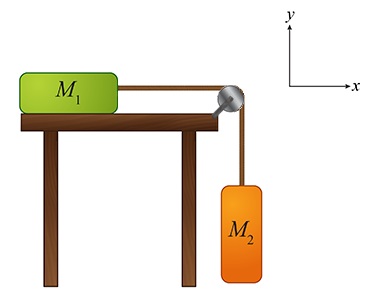
\includegraphics[width=0.25\textwidth]{figures/table.png}
\caption{\label{fig:blocks} Diagram for exercise 3, \textbf{Friction and Drag}.}
\end{figure}
\item A system of area $A$ moves at velocity $v$ through air with density $\rho_{air}$.  The drag force is $\vec{F}_D = \frac{1}{2}C\rho_{air} A v^2$, where $C$ is a measured constant.  (a) When weight $\vec{w}$ balances with $\vec{F}_D$, the system reaches \textit{terminal velocity} $v_{T}$.  Show that $v_T = \sqrt{2mg/C\rho A}$.  (b) What is $v_{T}$ for a skydiver who has $m=60$ kg, $A=1$ m$^2$, $C \approx 0.7$, in air with $\rho=1.225$ kg/m$^3$? (Use $v_T = \sqrt{2mg/C\rho A}$).
\end{enumerate}
\end{document}